% ULLAP journal manuscript, IEEE version (IEEEtran journal format).
% Same content as ullap_manuscript.tex (Elsevier): both input abstract.tex, body.tex and refs.bib,
% so edit the paper there and rebuild both. Red \TBD{} items are open before submission.
\documentclass[journal]{IEEEtran}
\usepackage{amsmath,amssymb}
\usepackage{graphicx}
\usepackage{booktabs}
\usepackage{multirow}
\usepackage{adjustbox}
\usepackage{xcolor}
\usepackage[hidelinks]{hyperref}
\graphicspath{{../results/plots/}}
\newcommand{\TBD}[1]{\textcolor{red}{[TBD: #1]}}
\newcommand{\WT}{table*}  % wide table spans both columns
\newcommand{\WF}{figure*} % wide figure spans both columns
\newcommand{\fitcol}[1]{\adjustbox{max width=\columnwidth}{#1}} % shrink a table to the column width

\begin{document}
\title{A Bit-Exact, Processor-Free FPGA Adaptive Noise Canceller: Fair Comparison of LMS, NLMS and
Divider-Free NLMS-Shift on Cyclone IV E}

\author{Satvik~Garg, Aditya~Gupta, and Jaffino~G%
\thanks{The authors are with the School of Electronics Engineering (SENSE), Vellore Institute of
Technology, Vellore, India. Corresponding author: Jaffino G. \TBD{e-mail and author order to be
confirmed by the authors}}}

\maketitle

\begin{abstract}
% Shared abstract (input by ullap_manuscript.tex, ullap_ieee.tex and ullap_cssp.tex); CSSP limit 150-250 words.
% The longer 27 Oct version is kept in abstract_long.tex.
Cancelling noise with a reference microphone is one of the oldest applications of the least-mean-square
(LMS) family, and a small field-programmable gate array (FPGA) can do it at audio rates with no processor
at all. We present ULLAP, a 12-bit, 32-tap noise canceller built for the DE2-115 board (Cyclone IV E) and
its WM8731 codec. A single serial core, sharing one multiplier, runs three algorithms: LMS, normalised LMS
(NLMS) with a restoring divider, and NLMS-Shift, in which a leading-one detector and a shift take the place
of the division. With step sizes tuned on held-out seeds, NLMS-Shift stays within the 95\% confidence
interval of NLMS on stationary and amplitude-step noise (22.37 and 24.33~dB over 20 seeds), beats LMS by
about 2~dB on amplitude steps, and needs 72 rather than 130 busy cycles per sample. We show that NLMS-Shift
is exactly NLMS with a level-dependent step lying between 0.5 and 1 times the nominal value. On real
recorded noise and speech the filters remove 11.7--14.9~dB and lift short-time objective intelligibility
from 0.69--0.78 to 0.95--0.98; with the speech taken out they remove 18.5--31.9~dB, so it is the speech,
not the noise, that sets the limit. A 12-bit word holds the quantisation loss under 0.4~dB on broadband
noise. On the board, every one of the 724,459 captured output samples from the three algorithms matches
the integer model, and the measured sample rate, latency and busy cycles agree with the
register-transfer-level design.

\end{abstract}

\begin{IEEEkeywords}
Adaptive noise cancellation, NLMS, divider-free normalisation, FPGA, fixed-point arithmetic,
bit-exact verification.
\end{IEEEkeywords}

% Shared manuscript body (input by ullap_manuscript.tex [Elsevier], ullap_ieee.tex [IEEE] and ullap_cssp.tex [Springer/CSSP]).
% Edit the paper here; \WT / \WF are table / figure environments that span both columns in the IEEE version;
% \fitcol{} shrinks a tabular to the column width there, \fitwide{} shrinks a wide table to the text width
% (both are no-ops in the CSSP version, whose sn-jnl tables do not take an adjustbox).
\providecommand{\decl}[1]{\noindent\textbf{#1.}\ } % run-in head of the declarations; restyled by ullap_cssp.tex
%--------------------------------------------------------------------------------------------
\section{Introduction}
Few places where people live or work are free of noise. An office air conditioner hums, a compressor runs
beside a production line, road noise fills a car cabin, and a hearing-aid user is surrounded by the
chatter of other people. If a second microphone can be placed near the noise source, the noise reaching
the main microphone can be predicted from this reference signal and subtracted. The predictor is an
adaptive filter: it learns the acoustic path between the two microphones while the system runs and
follows the path when it changes. For this filter, the least-mean-square (LMS) algorithm and its
normalized version (NLMS) remain the usual choice. Both cost only a few multiply--accumulate operations per
tap and per sample, and their behavior has been studied for decades~\cite{lu2021a}.

A small embedded device has to run this filter in real time, with a short and fixed delay and on very
little energy. A field-programmable gate array (FPGA) suits such a task well. The datapath can be shaped
around the algorithm, the latency is known to the clock cycle, and no processor or operating system is
needed for scheduling. In hardware, however, LMS and NLMS are not equally easy to build. LMS uses only
multipliers and adders, but its convergence speed depends on the input level. NLMS removes this
dependence by dividing the step size by the input power, at the price of one division per sample.
Dividers are slow and large, so recent designs approximate the division instead, with an approximate
Newton--Raphson iteration~\cite{guidotti2020}, with canonical-signed-digit reciprocals~\cite{yao2024}, or
with a binary reciprocal built from a leading-one detector and a shifter~\cite{huang2026}. The crudest
option is to round the input power to a power of two, after which the division is a plain shift. This
variant is called NLMS-Shift in the rest of the paper.

Two issues in the published work motivated this study. The first concerns tuning. Competing variants are
seldom tuned with equal care, so a reported gain can come from a weak baseline rather than from the
algorithm. An early version of the present work made exactly this mistake: NLMS-Shift looked 5.7~dB
better than NLMS until NLMS was given a sensible regularization constant, at which point the gap
vanished. The second issue is the link between model and silicon. Hardware papers usually report area,
clock rate and power. Such figures show that a design fits on the chip; they do not show that the chip
produces the same samples as the model behind the accuracy results.

This paper presents ULLAP, a 12-bit, 32-tap adaptive noise canceller for the low-cost Terasic DE2-115
board (Intel Cyclone IV E) and its WM8731 audio codec, and uses it to address both issues. The main
contributions are listed below.
\begin{enumerate}
\item \textbf{One serial core for three algorithms:} LMS, NLMS (with a restoring divider) and NLMS-Shift
run on the same serial core and share one multiplier, so the datapath, word length and filter length are
identical for all three. The core sits inside a complete audio system with no processor, closes timing at
50~MHz on Cyclone IV E, and is released together with all scripts and data.
\item \textbf{A fair comparison:} The step size and regularizer of every algorithm are chosen on held-out
seeds by one common rule, and each result carries a 20-seed 95\% confidence interval. Synthetic
scenarios, real recorded noise and speech, and a reproducible word-length study are all covered.
\item \textbf{A bit-exact verification chain:} The chain runs from a Python integer model through the RTL
to the board wrapper (86 regression tests, codec, freeze and reset behavior included). Captures of real
codec samples on the board show every output sample of all three algorithms to be identical to the model
output.
\item \textbf{Two explanations backed by measurement:} The first concerns the shift. NLMS-Shift turns out
to be NLMS with a step that moves between 0.5 and 1 times the nominal value as the input level changes.
Running NLMS with the average of that step reproduces NLMS-Shift within 0.3~dB on broadband noise; on
tonal input, however, the step jumps each time the window power crosses a power of two. The second
concerns the real recordings. Once the speech is taken out, the same filters remove 18.5--31.9~dB of the
same real noise, which means that the lower noise reduction with speech comes from the speech disturbing
the adaptation, not from the noise.
\end{enumerate}
The shift normalizer is not new, and no claim is made to it; Section~\ref{sec:related} places it among
earlier division-free designs.

The remainder of the paper is organized as follows. Section~\ref{sec:related} reviews the problem and
related work, and Section~\ref{sec:system} outlines the system. The algorithms and the fixed-point model
are described in Section~\ref{sec:model} and the hardware in Section~\ref{sec:hw}.
Sections~\ref{sec:verif} and~\ref{sec:setup} cover verification and the experimental set-up,
Section~\ref{sec:results} reports the results, and Sections~\ref{sec:disc} and~\ref{sec:concl} close the
paper with a discussion and conclusions.

%--------------------------------------------------------------------------------------------
\section{Literature review}\label{sec:related}
\subsection{The problem: noise in daily life}
Noise is now recognized as an environmental health risk, not just a nuisance. More than 113 million
people in Europe live with transport noise above 55~dB(A), and traffic noise alone is estimated to cost
about 1.3 million healthy life-years each year through its effects on the heart and blood
vessels~\cite{munzel2025}. Hahad et al.~\cite{hahad2025} reviewed the evidence linking long-term noise
exposure to mental-health disorders and discussed the biological pathways that may be responsible.
Hearing loss is the other half of the picture. The World Health Organization puts the number of people
living with some degree of hearing loss at about 1.5 billion and expects it to reach 2.5 billion by
2050~\cite{chadha2021}. For these listeners, background noise is the main reason speech stays hard to
follow, even with a hearing aid. Reducing noise at the microphone, or close to the ear, is useful beside
roads, where urban traffic noise lies mostly below 2~kHz~\cite{yang2024}; inside vehicle
cabins~\cite{jiang2023,zhu2024}; in ventilation ducts and air conditioners~\cite{zhu2025}; and in hearing
aids~\cite{yin2023,husstedt2023,tetteh2026}. Most of these devices are small, cheap and run on batteries,
so the processing must work in real time at low cost and low energy.

\subsection{Applications of adaptive noise control}
Yang et al.~\cite{yang2024} recorded road traffic noise at five sites in Beijing and built a feedforward
LMS prototype that removed close to 30~dB(A) of single- and dual-frequency noise below 2~kHz. For a
passenger car, Jiang et al.~\cite{jiang2023} made the FxLMS step size depend on the reference norm and
tuned the two parameters of this rule by particle-swarm optimization. Their system, running on a dSPACE
board, reached up to 12~dB below 100~Hz and about 3~dB over 20--400~Hz in road tests, against $-0.8$ to
0.3~dB for plain FxLMS. Zhu et al.~\cite{zhu2024} drove the car's own loudspeakers to control the first
four engine orders; the average reduction at 52 ear-level microphones was 6.2~dB, and 93\% of the
listeners in a jury test felt more comfortable with the system on. In hearing aids, Yin and
Chen~\cite{yin2023} weighted the error of a variable-step adaptive feedback canceller, which on a real
device converged 35\% faster than a PEM-IMLMS baseline and 60\% faster than PEM-NLMS. Husstedt et
al.~\cite{husstedt2023} measured six commercial behind-the-ear devices and found that impulse noise
reduction cuts C-weighted peak levels by up to 20~dB, about 9~dB on average. A recent systematic review of
speech enhancement for hearing aids~\cite{tetteh2026} concluded that deep networks do best in complex
acoustic scenes, while hybrids that keep an adaptive filter strike a better balance between latency and
computation on wearable devices.

\subsection{Adaptive algorithms}
Lu et al.\ surveyed a decade of active noise control algorithms in two parts, one on linear
systems~\cite{lu2021a} and one on nonlinear systems~\cite{lu2021b}. In both, LMS-type updates are still
the base on which most newer methods are built. One popular idea is to run a fast filter and an accurate
filter side by side and combine them. F\'elix et al.~\cite{felix2021} proposed a modified convex
combination of FXLMS filters that converged faster and attenuated more than both FXLMS and the earlier
convex scheme. Zhu et al.~\cite{zhu2025} joined an adaptive FxLMS filter and a CNN--GRU network through a
convex weight to cancel harmonic noise in a bent air-conditioner pipe. A different difficulty arises when
the loudspeaker leaks back into the reference microphone and the loop turns unstable; Li et
al.~\cite{li2024} handled this case with a Youla-parameterized feedforward controller and an adaptive IIR
update, tested on a duct. Each of these methods cancels better, but each adds operations, a network or a
whole extra filter to every sample, which runs against what a small FPGA design needs.

\subsection{Hardware realizations}
Thannoon and Hashim~\cite{thannoon2024} combined a fast retimed RLS filter with a slow LMS filter on an
FPGA to remove power-line interference from ECG records of the MIT-BIH database, and reported 24.2\%
higher SNR and 50\% faster convergence than conventional structures. Jagadeeswari et
al.~\cite{jagadeeswari2026} applied cut-set retiming to delayed NLMS filters for audio on a Spartan-6 and
shortened the critical path from 29.96 to 13.39~ns. For underwater sonar, Karakaya and
Aytar~\cite{karakaya2026} built semi-parallel 16-bit NLMS and variable-step LMS filters on an Artix-7;
the SNR rose from 8.85~dB to 29.36 and 28.57~dB, respectively, while using 2.51\% and 2.91\% of the LUTs.
Park and Park~\cite{park2023} took another route, letting a small CNN classify the noise and pick one of
several fixed filters, which in simulation gave 2.3~dB more SNR than LMS with 53\% less dynamic power.
Abdi et al.~\cite{abdi2024} designed a narrowband controller around a variable-step LMS notch filter on an
FPGA to suppress microphonics in a superconducting accelerator cavity. Other groups worked on the
arithmetic. Nagabushanam et al.~\cite{nagabushanam2025} built a multiplier-less LMS filter from
distributed arithmetic with offset-binary coding, and da Rosa et al.~\cite{rosa2022} replaced the
multipliers of an LMS power-line canceller with adders and shifters, saving up to 4.98 times in power and
30.46\% in area.

\subsection{Removing the division from NLMS}
Closest to the present study are the papers that attack the NLMS division itself. Guidotti et
al.~\cite{guidotti2020} saved power in an NLMS interference canceller with an approximate Newton--Raphson
integer divider, and Coelho et al.~\cite{coelho2022} reduced the cost of adaptive filtering with
sum-of-powers-of-two arithmetic. Yao and Huang~\cite{yao2024} approximated the reciprocal of the input
power by canonical-signed-digit encoded divisors in a 16-tap NLMS FIR filter. Huang and
Yao~\cite{huang2026} followed with a binary reciprocal approximation for an NLMS IIR filter. On the same
DE2-115 board used here, their design needs 5.07~nJ per sample, compared with 8.33~nJ for a 15-bit SRT
divider, and lowers the energy per sample by 39.1\%, 6.5\%, 14.4\% and 5.6\% relative to the SRT,
Newton--Raphson, CSD and lookup-table methods~\cite{huang2026}. They also remark that the older idea of
rounding the divisor to a single power of two, so that the division becomes a shift, suffers from a large
approximation error. That plain shift is exactly NLMS-Shift. Section~\ref{sec:equiv} shows that its error
acts only as a level-dependent step factor between 0.5 and 1.

No study was found that compares LMS, a true divider and a shift normalizer on a single core with equal
tuning and statistical tests, and only a few test a complete audio system with a codec on a board. ULLAP
contributes this equal-effort three-way comparison, a bit-exact chain from model to hardware, and an
evaluation on real recordings.

%--------------------------------------------------------------------------------------------
\section{System overview}\label{sec:system}
Fig.~\ref{fig:system} gives an overview of the system. Noise from the source $v$ reaches the primary
microphone through an unknown acoustic path $h$ and mixes there with the wanted signal $s$, while a
reference microphone close to the source picks up $v$ directly. The two microphones feed the left and
right LINE IN channels of the WM8731 codec, which digitizes both signals and sends them to the FPGA over
an I$^2$S link. Inside the FPGA, the I$^2$S receiver hands one pair $(x[n],d[n])$ to the ANC core in every
sample period. The core returns the error $e[n]$, that is, the cleaned signal, and the I$^2$S transmitter
passes it back to the codec DAC and LINE OUT. An I$^2$C engine programs the codec once after reset. Two
slide switches select bypass and freeze the adaptation, a push button resets the system, and four GPIO
test points bring out the sample strobe, the output strobe, the busy flag and the frame clock so that the
timing can be measured. The whole design is plain Verilog, with no processor and no vendor IP.

\begin{\WF}[!htbp]\centering
\adjustbox{max width=\linewidth}{%
% Fig. (system block diagram), input by body.tex inside an adjustbox that scales it to the text width.
\begin{tikzpicture}[font=\fontsize{8}{9.5}\selectfont, >=Stealth,
  blk/.style={draw, rounded corners=2pt, align=center, minimum height=8mm, inner sep=3pt, fill=white},
  core/.style={blk, fill=gray!15, line width=0.8pt, minimum width=25mm},
  lab/.style={font=\fontsize{7}{8}\selectfont, inner sep=1.5pt}]
  % acoustic part
  \node[blk] (src)  at (0,-1.6)   {Noise\\source $v[n]$};
  \node[blk] (path) at (2.0,-0.4) {Acoustic\\path $h$};
  \node[draw, circle, inner sep=1pt] (sum) at (3.45,-0.4) {$+$};
  \node[blk] (spk)  at (3.45,0.9) {Speech $s[n]$};
  \node[blk] (pmic) at (4.95,-0.4) {Primary\\mic};
  \node[blk] (rmic) at (4.95,-2.8) {Reference\\mic};
  \draw[->] (src.north) |- (path.west);
  \draw[->] (src.south) |- (rmic.west);
  \draw[->] (path) -- (sum);
  \draw[->] (spk) -- (sum);
  \draw[->] (sum) -- (pmic);
  % codec
  \node[blk, minimum height=32mm, minimum width=15mm] (adc) at (7.0,-1.6) {WM8731\\ADC};
  \draw[->] (pmic) -- node[lab, above]{$d$} (pmic -| adc.west);
  \draw[->] (rmic) -- node[lab, above]{$x$} (rmic -| adc.west);
  \node[blk, minimum width=15mm] (dac) at (7.0,-7.3) {WM8731\\DAC};
  \node[blk] (out) at (4.95,-7.3) {LINE OUT\\$e[n]$};
  % FPGA, main signal path top to bottom
  \node[blk, minimum width=15mm] (rx)  at (10.3,-1.6) {I$^2$S RX};
  \node[core] (anc) at (10.3,-3.6) {ANC core\\LMS / NLMS /\\NLMS-Shift};
  \node[blk, minimum width=15mm] (mux) at (10.3,-5.6) {Bypass\\mux};
  \node[blk, minimum width=15mm] (tx)  at (10.3,-7.3) {I$^2$S TX};
  \draw[->] (adc.east |- rx) -- node[lab, above]{I$^2$S} (rx);
  \draw[->] (rx) -- node[lab, right]{$x$, $d$} (anc);
  \draw[->] (anc) -- node[lab, right]{$e$} (mux);
  \draw[->] (mux) -- (tx);
  \draw[->] (tx) -- (dac);
  \draw[->] (dac) -- (out);
  % bypass path on the left of the main column
  \draw[->] ([xshift=-3mm]rx.south) -- ++(0,-0.35) -| (8.65,-4.9) |- ([yshift=1.5mm]mux.west);
  \node[lab, rotate=90] at (8.85,-3.6) {$d$ (bypass)};
  % side blocks
  \node[blk, minimum width=18mm] (i2c)  at (13.9,-1.6) {I$^2$C\\config};
  \node[blk, minimum width=18mm] (gpio) at (13.9,-3.6) {GPIO\\test points};
  \node[blk, minimum width=18mm] (sync) at (13.9,-5.6) {Synchro-\\nizers};
  \draw[->] (i2c.north) -- ++(0,1.65) -| (adc.north);
  \draw[->] (anc.east) -- node[lab, above]{strobes} (gpio.west);
  \draw[->] ([yshift=2mm]sync.west) -| node[lab, above, pos=0.25]{freeze} ([xshift=10.5mm]anc.south);
  \draw[->] ([yshift=-2mm]sync.west) -- node[lab, below]{bypass} ([yshift=-2mm]sync.west -| mux.east);
  \node[blk] (sw) at (13.9,-8.6) {SW[1:0], KEY0};
  \draw[->] (sw) -- (sync);
  \coordinate (bpl) at (8.55,-4.9);
  \begin{scope}[on background layer]
    \node[draw, dashed, rounded corners, fit=(rx)(anc)(mux)(tx)(i2c)(gpio)(sync)(bpl), inner sep=8pt,
      label={[font=\fontsize{8}{9.5}\selectfont, anchor=south west, inner sep=2pt]north west:FPGA (Cyclone IV E, 50~MHz)}] (fpga) {};
  \end{scope}
\end{tikzpicture}
}
\caption{Block diagram of the ULLAP system. In the experiments the acoustic part (upper left) is
simulated (Section~\ref{sec:setup}); everything from the codec onwards runs on the DE2-115 board.}\label{fig:system}
\end{\WF}

%--------------------------------------------------------------------------------------------
\section{Algorithms and fixed-point model}\label{sec:model}
\subsection{Signal model and cost function}
The reference microphone hears only the noise. The primary microphone hears the speech, the noise after
the acoustic path, and a little sensor noise $n_s$:
\begin{align}
x[n] &= v[n], \label{eq:x}\\
d[n] &= s[n] + \sum_{j=0}^{M-1} h_j\, v[n-j] + n_s[n]. \label{eq:d}
\end{align}
With the last $L$ reference samples collected in $\mathbf{x}[n]=[x[n],\dots,x[n-L+1]]^T$ and the weights
in $\mathbf{w}[n]=[w_0[n],\dots,w_{L-1}[n]]^T$, the filter estimates the noise part of $d[n]$, and
whatever remains is the system output:
\begin{align}
y[n] &= \mathbf{w}^T[n]\,\mathbf{x}[n] = \sum_{i=0}^{L-1} w_i[n]\,x[n-i], \label{eq:y}\\
e[n] &= d[n]-y[n]. \label{eq:e}
\end{align}
Because $s$ is uncorrelated with $v$, minimizing the mean-square error
\begin{align}
J(\mathbf{w}) &= E\{e^2[n]\} = E\{d^2[n]\} - 2\,\mathbf{w}^T\mathbf{p} + \mathbf{w}^T\mathbf{R}\,\mathbf{w}, \label{eq:J}\\
\mathbf{R} &= E\{\mathbf{x}[n]\,\mathbf{x}^T[n]\},\qquad \mathbf{p}=E\{d[n]\,\mathbf{x}[n]\}, \label{eq:Rp}
\end{align}
removes the noise and leaves the speech untouched. Here $\mathbf{R}$ is the autocorrelation matrix of the
reference vector and $\mathbf{p}$ the cross-correlation between $d[n]$ and $\mathbf{x}[n]$. The minimum
lies at the Wiener solution $\mathbf{w}_o=\mathbf{R}^{-1}\mathbf{p}$, which coincides with the acoustic
path when $L\ge M$ and $n_s$ is white.

\subsection{LMS, NLMS and NLMS-Shift}
LMS replaces the gradient $\nabla J=-2(\mathbf{p}-\mathbf{R}\mathbf{w})$ by its instantaneous estimate
$-2e[n]\mathbf{x}[n]$, which leads to the update shared by all three algorithms:
\begin{equation}
\mathbf{w}[n+1]=\mathbf{w}[n]+\mu[n]\,e[n]\,\mathbf{x}[n].
\label{eq:upd}
\end{equation}
Only the step $\mu[n]$ differs. Writing the window power as $P[n]=\|\mathbf{x}[n]\|^2$, the steps of LMS,
NLMS and NLMS-Shift are
\begin{align}
\mu_{\text{LMS}}[n] &= \mu, & 0<\mu&<\frac{2}{L\,\sigma_x^2}, \label{eq:mu_lms}\\
\mu_{\text{NLMS}}[n] &= \frac{\tilde\mu}{P[n]+\epsilon}, & 0<\tilde\mu&<2, \label{eq:mu_nlms}\\
\mu_{\text{Shift}}[n] &= 2^{-(k[n]+K)}, && \label{eq:mu_shift}\\
k[n] &= \lfloor\log_2(P[n]+\epsilon)\rfloor+1, && \label{eq:k}
\end{align}
where $\sigma_x^2$ is the reference variance and $\epsilon>0$ a small regularizer. The LMS bound moves
with the input level, which is why a fixed $\mu$ ends up too slow for quiet inputs or unstable for loud
ones. The NLMS bound stays put. The hardware keeps the power up to date through the exact recursion
\begin{equation}
P[n] = P[n-1] + x^2[n] - x^2[n-L],
\label{eq:prec}
\end{equation}
which costs two squarings per sample instead of $L$. In NLMS-Shift the exponent $k[n]$ is just the bit
length of $P[n]+\epsilon$. A leading-one detector finds it, and multiplying by $\mu[n]$ reduces to an
arithmetic right shift of $e[n]\,x[n-i]$ by $k[n]+K$ places.

\begin{proposition}\label{prop:bound}
For every $n$, the NLMS-Shift step \eqref{eq:mu_shift} satisfies
\begin{equation}
\frac{2^{-K}}{2\,(P[n]+\epsilon)} \;\le\; \mu_{\text{Shift}}[n] \;<\; \frac{2^{-K}}{P[n]+\epsilon},
\label{eq:bound}
\end{equation}
Put differently, the NLMS-Shift step is never more than a factor of two below the NLMS step with
$\tilde\mu=2^{-K}$, and it stays inside the NLMS stability bound $0<\tilde\mu<2$ whenever $K\ge0$.
\end{proposition}
\noindent\emph{Proof.} By \eqref{eq:k}, $2^{k[n]-1}\le P[n]+\epsilon<2^{k[n]}$. Taking reciprocals and
multiplying by $2^{-K}$ gives \eqref{eq:bound}, since $\mu_{\text{Shift}}[n]=2^{-K}\,2^{-k[n]}$.\hfill$\square$

\smallskip\noindent More precisely, the two steps are related by
\begin{equation}
\mu[n]=\frac{r[n]\,2^{-K}}{P[n]+\epsilon},\qquad
r[n]=\frac{P[n]+\epsilon}{2^{\lfloor\log_2(P[n]+\epsilon)\rfloor+1}}\in[0.5,1),
\label{eq:ratio}
\end{equation}
so NLMS-Shift is simply NLMS with the time-varying step $2^{-K}r[n]$ (Section~\ref{sec:equiv}). When the
input level is unknown over several octaves, the fractional part
$u=\log_2(P+\epsilon)-\lfloor\log_2(P+\epsilon)\rfloor$ is spread evenly over $[0,1)$, and the ratio
averages to
\begin{equation}
E\{r\}=\int_0^1 2^{u-1}\,du=\frac{1}{2\ln 2}\approx 0.72 .
\label{eq:er}
\end{equation}

\subsection{Fixed-point model}
Signals and weights are signed $Q1.F$ numbers with $W=12$ bits and $F=W-1$ fraction bits. With the
rounding shift and the saturation
\begin{align}
\operatorname{rs}(a,m) &= \left\lfloor \frac{a+2^{m-1}}{2^m}\right\rfloor, \label{eq:rs}\\
\operatorname{sat}_B(a) &= \min\!\left(\max\!\left(a,-2^{B-1}\right),\,2^{B-1}-1\right), \label{eq:sat}
\end{align}
the integer datapath processes the samples $x_i=x[n-i]\cdot2^F$ and weights $w_i$ as
\begin{align}
a[n] &= \operatorname{sat}_{B_a}\Big(\sum_{i=0}^{L-1} w_i\,x_i\Big), \label{eq:acc}\\
B_a &= 2W+\lceil\log_2 L\rceil, \label{eq:ba}\\
y[n] &= \operatorname{sat}_W\big(\operatorname{rs}(a[n],F)\big), \label{eq:yq}\\
e[n] &= \operatorname{sat}_W\big(d[n]-y[n]\big), \label{eq:ye}\\
w_i &\leftarrow \operatorname{sat}_W\big(w_i+\Delta w_i\big), \label{eq:wupd}
\end{align}
and the weight increments of LMS, NLMS and NLMS-Shift are
\begin{align}
\Delta w_i^{\text{LMS}} &= \operatorname{rs}\big((M_\mu\,e[n])\,x_i,\;F+10\big), \label{eq:dw_lms}\\
\Delta w_i^{\text{NLMS}} &= \operatorname{rs}\big(g[n]\,x_i,\;F\big), \label{eq:dw_nlms}\\
g[n] &= \operatorname{sat}_{W+4}\!\left(\left\lfloor\frac{2N[n]+Q[n]}{2Q[n]}\right\rfloor\right), \label{eq:g}\\
\Delta w_i^{\text{Shift}} &= \operatorname{rs}\big(e[n]\,x_i,\;b(Q[n])-F+K\big), \label{eq:dw_shift}
\end{align}
Here $\mu=M_\mu\,2^{-10}$, $N[n]=M_\mu\,e[n]\,2^{2F-10}$, $Q[n]=P[n]+2^{2F-E}$ for $\epsilon=2^{-E}$, and
$b(\cdot)$ is the bit length of a positive integer. Wherever a value is narrowed, it saturates and sets a
sticky flag, so no overflow can pass unnoticed. The integer model (\texttt{py/fixedpoint.py},
\texttt{py/rtl\_model.py}) uses exactly these widths and produces the golden vectors.

%--------------------------------------------------------------------------------------------
\section{Hardware architecture}\label{sec:hw}
\subsection{Core}\label{sec:core}
Fig.~\ref{fig:core} shows the core datapath (\texttt{rtl/anc\_core.v}, vendor-neutral Verilog). The core
takes one sample pair per \texttt{in\_valid} strobe and does all of its arithmetic on one multiplier with a
three-stage pipeline (operand registers, product register, consume stage). A finite-state machine walks
through each sample: two cycles square the new and the dropped reference samples for \eqref{eq:prec}
(NLMS and NLMS-Shift only), $L$ cycles form the filter sum \eqref{eq:acc}, and one cycle produces $y$ and
$e$ \eqref{eq:ye}. The step computation comes next, followed by $L$ cycles of weight updates
\eqref{eq:wupd}. For the gain $g[n]$, NLMS adds a sequential restoring divider; NLMS-Shift has a
leading-one detector and a shift-amount register instead. A \texttt{freeze} input holds the weights while
filtering continues.

\begin{\WF}[!htbp]\centering
\adjustbox{max width=\linewidth}{%
% Fig. (ANC core datapath), input by body.tex inside an adjustbox that scales it to the text width.
\begin{tikzpicture}[font=\fontsize{8}{9.5}\selectfont, >=Stealth,
  blk/.style={draw, rounded corners=2pt, align=center, minimum height=8mm, inner sep=3pt, fill=white},
  reg/.style={draw, align=center, minimum height=8mm, minimum width=27mm, inner sep=3pt, fill=gray!10},
  lab/.style={font=\fontsize{7}{8}\selectfont, inner sep=1.5pt}]
  % storage on the left
  \node[reg] (xv) at (0,1.7)  {Tap delay line\\$x[n],\dots,x[n-L+1]$};
  \node[reg] (wv) at (0,-0.5) {Weight registers\\$w_0,\dots,w_{L-1}$};
  \node (xin) at (0,3.3) {$x[n]$};
  \draw[->] (xin) -- (xv.north);
  % shared arithmetic
  \node[blk] (opm) at (3.05,0.6) {Operand\\mux};
  \node[blk] (mul) at (5.6,0.6) {Multiplier\\(3-stage pipeline)};
  \draw[->] (xv.east) -- ++(0.3,0) |- ([yshift=1.5mm]opm.west);
  \draw[->] (wv.east) -- ++(0.65,0) |- ([yshift=-1.5mm]opm.west);
  \draw[->] (opm) -- (mul);
  % consumers of the product
  \node[blk, minimum width=20mm] (acc) at (8.85,2.5)  {Accumulator\\$a[n]$};
  \node[blk, minimum width=20mm] (pw)  at (8.85,0.6)  {Power\\$P[n]$ \eqref{eq:prec}};
  \node[blk, minimum width=20mm] (upd) at (8.85,-1.3) {Update\\$\operatorname{rs}$, $\operatorname{sat}_W$};
  \coordinate (bus) at (7.35,0.6);
  \draw (mul.east) -- (bus);
  \fill (bus) circle (1.2pt);
  \draw[->] (bus) |- (acc.west);
  \draw[->] (bus) -- (pw.west);
  \draw[->] (bus) |- (upd.west);
  % output stage and step unit
  \node[blk, minimum width=25mm] (ye) at (11.75,2.5) {Round, saturate\\$y$, $e=d-y$};
  \node[blk, minimum width=25mm, fill=gray!15] (norm) at (11.75,0.45) {Step unit\\LMS: $M_\mu$\\NLMS: divider\\Shift: LOD $\to k$};
  \draw[->] (acc) -- (ye);
  \draw[->] (pw) -- (pw -| norm.west);
  \draw[->] (norm.south) |- node[lab, below, pos=0.75]{shift $k+K$} (upd.east);
  \draw[->] ([yshift=-1.5mm]ye.east) -- ++(0.7,0) node[right, inner sep=1pt]{$e[n]$};
  \node (din) at (12.4,4.0) {$d[n]$};
  \draw[->] (din) -- (din |- ye.north);
  \draw[->] ([xshift=-6.5mm]ye.north) -- ++(0,0.75) -| node[lab, above, pos=0.25]{$e$, $M_\mu e$, $g$ to operand mux} (opm.north);
  % weight write-back
  \draw[->] (upd.south) -- ++(0,-0.75) -| (wv.south);
  % control
  \node[blk, minimum width=31mm] (fsm) at (4.3,-1.05) {Control FSM\\IDLE, P0, P1, MAC, YE,\\MU, DIV, UPD, WAIT};
  \draw[->, dashed] (fsm.north -| opm.south) -- (opm.south);
  \draw[->, dashed] (fsm.north -| mul.south) -- (mul.south);
  \draw[->, dashed] ([xshift=8mm]fsm.south) |- (13.55,-2.35) |- (norm.east);
\end{tikzpicture}
}
\caption{Datapath of the ANC core. The power update, filter sum, step computation and weight updates all
share one multiplier; the three algorithms differ only in the step unit. Dashed lines are control
signals.}\label{fig:core}
\end{\WF}

With this schedule, the input-to-output latency and the number of busy cycles per sample are fixed:
\begin{align}
N_{\text{lat}} &= \begin{cases} L+3 & \text{LMS},\\ L+5 & \text{NLMS, NLMS-Shift},\end{cases} \label{eq:lat}\\
N_{\text{busy}} &= \begin{cases} 2L+9 & \text{LMS},\\ 2L+13+N_{\text{div}} & \text{NLMS},\\ 2L+8 & \text{NLMS-Shift},\end{cases} \label{eq:busy}
\end{align}
The restoring divider takes one iteration per dividend bit,
$N_{\text{div}}=W+B_\mu+2F+4+\lceil\log_2 L\rceil$, with $B_\mu$ the signed width of $M_\mu$, so the NLMS
cycle count grows with the step-size constant. For $L=32$ and the tuned settings, the formulas give
latencies of 35, 37 and 37 cycles and busy times of 73, 130 ($N_{\text{div}}=53$) and 72 cycles, exactly
the values measured on the board (Section~\ref{sec:board}).

\subsection{Board wrapper}
Around the core, the DE2-115 wrapper holds an I$^2$C engine that configures the WM8731 at reset (11
registers, every write acknowledge-checked), an I$^2$S receiver and transmitter, two-flop synchronizers on
the reset and switches, a frame-latched bypass multiplexer, an overrun flag, and four registered test
points on the GPIO header. The I$^2$S blocks run on the 50~MHz system clock and treat the codec's bit and
word clocks as data. The codec is the clock master. It is driven from a 12.5~MHz clock with its
sample-rate register at 1536~fs, which sets the sample rate and the number of clock cycles per sample to
\begin{align}
f_s &= \frac{f_{\text{MCLK}}}{1536}=\frac{12.5~\text{MHz}}{1536}=8.138~\text{kHz}, \label{eq:fs}\\
N_s &= \frac{f_{\text{clk}}}{f_s}=\frac{50~\text{MHz}}{8.138~\text{kHz}}=6144, \label{eq:ns}
\end{align}
where $f_s$ is also the rate used in the simulations. The core is busy for the fraction
\begin{equation}
U=\frac{N_{\text{busy}}}{N_s}
\label{eq:util}
\end{equation}
of every sample period; by \eqref{eq:busy} that is 1.19\%, 2.12\% and 1.17\% for LMS, NLMS and
NLMS-Shift. Again, no processor or vendor IP is involved.

%--------------------------------------------------------------------------------------------
\section{Verification}\label{sec:verif}
Verification was done at three levels, and Table~\ref{tab:verif} lists what was run. At the core level,
golden vectors from the integer model cover 68 configurations: word lengths $W$ of 8 to 31 bits, filter
lengths $L$ of 2 to 32 taps, saturation corner cases and several freeze patterns. For each of them the
testbench checks every $y[n]$ and $e[n]$, the final weights, the sticky flags and the latency. One level
up, the top-level testbench places the board design around a behavioral model of the WM8731. This model
checks each I$^2$C write and runs at whatever sample rate has been programmed, and tests T1--T10 exercise
configuration, NACK handling, bypass, end-to-end cancellation against golden vectors, freeze, reset, the
flags, the clocks, a 45-point skew sweep, the 8~kHz rate and the GPIO timing. A testbench that passes is
only useful if it is able to fail, so faults were planted in the RTL on purpose (mutation testing); each
of them was caught. Verilator, run with \texttt{-Wall}, gives no unwaived warning. The third level, the
board itself, is covered in Section~\ref{sec:board}.

\begin{table}[!htbp]\centering\small
\caption{Verification summary. All RTL suites pass in both Icarus Verilog and Questa
(\texttt{results/metrics/iverilog\_regression\_summary.txt}, \texttt{results/local\_run\_da0b6f4/}).}\label{tab:verif}
\fitcol{\begin{tabular}{lrl}\toprule
Suite & Tests & Result\\\midrule
Core golden vectors (\texttt{tb\_anc\_core}) & 68 & all pass, bit-exact\\
Protocol corner cases & 4 & pass\\
Freeze hold/toggle variants & 3 & pass\\
Top level with codec model (T1--T10) & 11 & pass\\
Python unit tests & 53 & pass\\
Verilator lint (\texttt{-Wall}) & -- & 0 unwaived\\
On-board Signal Tap captures (T9) & 25 & all bit-exact\\
On-board freeze, DAC word, 10-min soak & 4 & pass\\\bottomrule
\end{tabular}}
\end{table}

%--------------------------------------------------------------------------------------------
\section{Experimental set-up}\label{sec:setup}
All synthetic runs follow the reference model $x=v$, $d=s+h*v+n_s$, sampled at 8~kHz, with 16,000
samples per run. Four scenarios are used: stationary colored noise; amplitude steps, in which the noise is
scaled by $\times3$ and later by $\times0.25$; an acoustic path that switches abruptly at the midpoint; and
a recorded chord as the noise source. Tuning was done on separate seeds (101--103). For each algorithm,
the step size and regularizer were picked to give the highest mean final noise reduction over the
stationary, amplitude-step and path-switch scenarios, and any setting that overflowed was discarded. This
led to $\mu=0.25$ for LMS, $\mu=0.25$ with $\epsilon=1$ for NLMS, and $K=3$ with $\epsilon=0.25$ for
NLMS-Shift. Seeds 1--20, which played no part in tuning, produced every result reported below. The final
noise reduction is computed over the last quarter $\mathcal{N}$ of each run,
\begin{equation}
\mathrm{NR}=10\log_{10}\frac{\sum_{n\in\mathcal{N}}\big(d[n]-s[n]\big)^2}{\sum_{n\in\mathcal{N}}\big(e[n]-s[n]\big)^2}\ \text{dB},
\label{eq:nr}
\end{equation}
and the tables give its mean over the $S=20$ seeds together with a 95\% confidence interval,
\begin{equation}
\overline{\mathrm{NR}}\pm t_{0.975,\,S-1}\,\frac{\sigma_{\mathrm{NR}}}{\sqrt{S}},\qquad t_{0.975,19}=2.093 .
\label{eq:ci}
\end{equation}
When two algorithms A and B are compared, the test works on the per-seed differences
$\Delta_k=\mathrm{NR}_{\mathrm{A},k}-\mathrm{NR}_{\mathrm{B},k}$, since both algorithms see the same noise
realizations. A and B count as equivalent if two one-sided tests (TOST) at $p<0.05$ both rule out a mean
difference beyond $\pm\delta$, with $\delta=0.5$~dB; that is, if both null hypotheses
\begin{equation}
H_{01}:\ \bar\Delta\le-\delta,\qquad H_{02}:\ \bar\Delta\ge\delta .
\label{eq:tost}
\end{equation}
are rejected.

\emph{Use of generative AI.} The authors used Claude (Anthropic) as an assistant during this work: for
writing and debugging the analysis scripts and testbench code, for searching and summarizing the
literature, and for drafting and editing the manuscript text. \TBD{Authors: add any other AI tools you used (for example
for local runs or literature searches) and adjust the list above if needed.} Every reported number was
checked by the authors against the committed result files and board captures, each reference was checked
against its source, and the authors take full responsibility for the content of this article.

The real-audio test uses material from the public MS-SNSD
corpus\footnote{\url{https://github.com/microsoft/MS-SNSD}}: four noise recordings (an air conditioner, a
vacuum cleaner, a copy machine and babble) and ten utterances, all resampled to 8~kHz. For every seed, a
noise segment, an utterance and a random 16-tap acoustic path are drawn and mixed at 0~dB input SNR. Each
mix is processed twice, once with a clean reference and once with the speech leaking into the reference
at $-20$~dB. The first 2~s are left for convergence, and the noise reduction, the short-time objective
intelligibility measure (STOI) and the narrow-band perceptual evaluation of speech quality (PESQ, ITU-T
Recommendation P.862) are computed on the rest.

%--------------------------------------------------------------------------------------------
\section{Results}\label{sec:results}
\subsection{Synthetic scenarios}
\begin{\WT}[!htbp]\centering\small
\caption{Final noise reduction, dB, mean [95\% CI] over seeds 1--20, $W=12$, $L=32$ (\texttt{results/paper\_numbers.csv}).}\label{tab:nr}
\begin{tabular}{lccc}\toprule
Scenario & LMS & NLMS & NLMS-Shift\\\midrule
Stationary   & 22.39 [22.12, 22.66] & 22.28 [22.01, 22.54] & 22.37 [22.11, 22.63]\\
Amplitude steps & 22.36 [21.72, 23.00] & 24.16 [23.58, 24.73] & 24.33 [23.88, 24.78]\\
Path switch  & 18.95 [18.81, 19.09] & 18.53 [18.39, 18.67] & 18.91 [18.76, 19.06]\\
Recorded chord & 5.69 [5.66, 5.73] & 5.73 [5.69, 5.76] & 5.46 [5.42, 5.50]\\\bottomrule
\end{tabular}
\end{\WT}
The final noise reduction of the three algorithms is listed in Table~\ref{tab:nr}. NLMS-Shift and NLMS
come out level on stationary noise and on amplitude steps, and NLMS-Shift and LMS come out level on
stationary noise and on the path switch. Amplitude steps are where LMS falls behind: both normalized
algorithms are about 2~dB better there. With a fixed step, LMS is caught between two bad options,
adapting too slowly after the drop or too noisily before it. Fig.~\ref{fig:pareto} makes the trade-off
visible. No LMS step size gives 22~dB on stationary noise and 24~dB on amplitude steps at the same time,
while both NLMS variants manage it. The recorded chord is the one case in which NLMS-Shift loses ground,
by 0.2--0.3~dB.

What counts as a tie is settled by the paired per-seed tests in Table~\ref{tab:paired}. Every difference
between NLMS-Shift and NLMS lies inside the $\pm0.5$~dB equivalence margin (TOST, $p<0.05$). Some of
these differences are still statistically non-zero, the $+0.38$~dB on the path switch being one example,
but they are small enough to count as ties. Against LMS on amplitude steps, the 1.8--2.0~dB lead of the
normalized algorithms is significant ($p<10^{-7}$).

\begin{\WT}[!htbp]\centering\scriptsize
\caption{Paired differences in final NR over seeds 1--20 (\texttt{results/metrics/paired\_stats.csv}).}\label{tab:paired}
\fitwide{\begin{tabular}{llcccc}\toprule
Scenario & Pair & Mean diff. (dB) & 95\% CI & $p$ (paired $t$) & TOST $\pm$0.5 dB\\\midrule
Stationary & NLMS-Shift $-$ NLMS & +0.10 & [+0.01, +0.18] & 0.028 & equivalent\\
Stationary & NLMS-Shift $-$ LMS & -0.02 & [-0.07, +0.04] & 0.58 & equivalent\\
Stationary & NLMS $-$ LMS & -0.11 & [-0.18, -0.04] & 0.0038 & equivalent\\
Amplitude steps & NLMS-Shift $-$ NLMS & +0.17 & [-0.12, +0.47] & 0.23 & equivalent\\
Amplitude steps & NLMS-Shift $-$ LMS & +1.97 & [+1.51, +2.43] & 2.8e-08 & not equiv.\\
Amplitude steps & NLMS $-$ LMS & +1.79 & [+1.38, +2.21] & 2.5e-08 & not equiv.\\
Path switch & NLMS-Shift $-$ NLMS & +0.38 & [+0.30, +0.47] & 1.9e-08 & equivalent\\
Path switch & NLMS-Shift $-$ LMS & -0.04 & [-0.07, -0.01] & 0.018 & equivalent\\
Path switch & NLMS $-$ LMS & -0.42 & [-0.50, -0.34] & 1.1e-09 & equivalent\\
Recorded chord & NLMS-Shift $-$ NLMS & -0.27 & [-0.30, -0.24] & 7.7e-14 & equivalent\\
Recorded chord & NLMS-Shift $-$ LMS & -0.24 & [-0.26, -0.22] & 2.6e-16 & equivalent\\
Recorded chord & NLMS $-$ LMS & +0.03 & [+0.00, +0.06] & 0.036 & equivalent\\
\bottomrule\end{tabular}
}
\end{\WT}

\begin{\WF}[!htbp]\centering
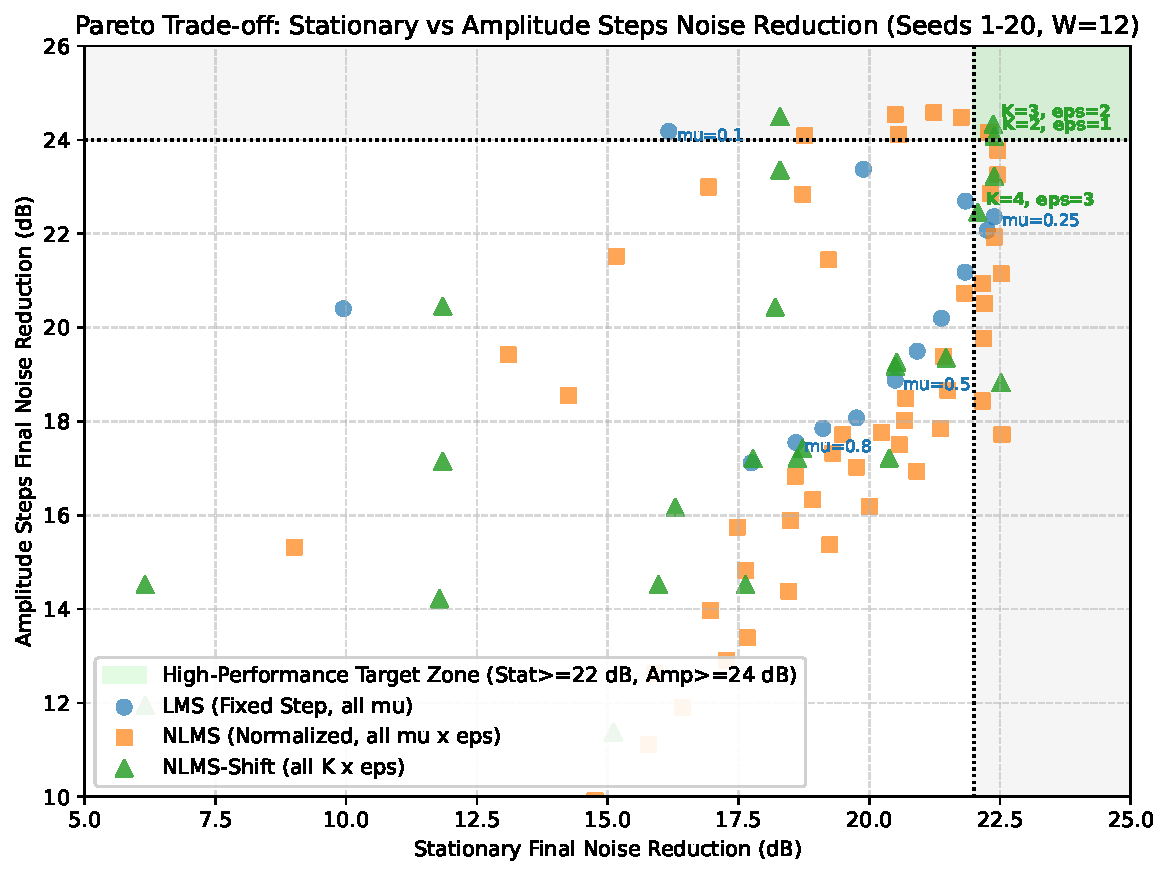
\includegraphics[width=0.75\linewidth]{fig12_pareto_stationary_amp_steps.pdf}
\caption{Noise reduction on stationary noise against that on amplitude steps over a range of step sizes (seeds 1--20).}\label{fig:pareto}
\end{\WF}

Figs.~\ref{fig:conv}--\ref{fig:track} follow a single run (seed~1) at the fair-tuned settings.
Fig.~\ref{fig:conv} plots the running noise reduction in each scenario, Fig.~\ref{fig:resid} sets the
residual error power against the input noise power for stationary noise, and Fig.~\ref{fig:track} shows
how each algorithm responds to the amplitude steps. The drop at 1.2~s is the telling moment: after it,
LMS settles roughly 3~dB under the two normalized algorithms, consistent with Table~\ref{tab:nr}.

\begin{\WF}[!htbp]\centering
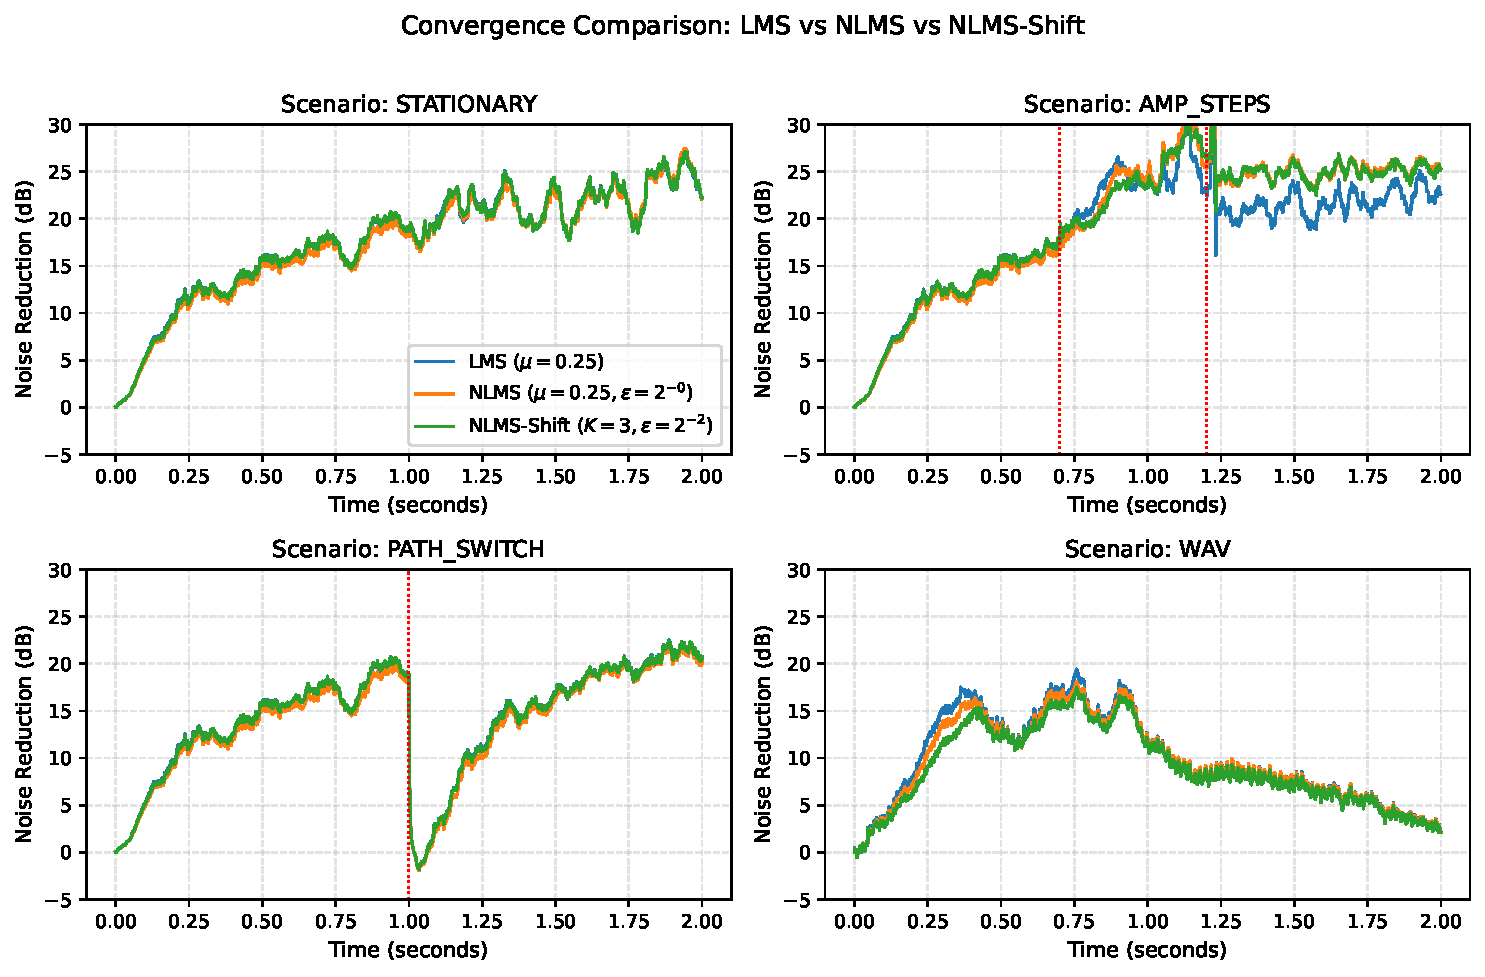
\includegraphics[width=0.9\linewidth]{fig1_convergence_paper.pdf}
\caption{Running noise reduction in the four synthetic scenarios (seed 1, $W=12$, $L=32$, fair-tuned settings). Dotted lines mark the amplitude steps and the path switch.}\label{fig:conv}
\end{\WF}
\begin{figure}[!htbp]\centering
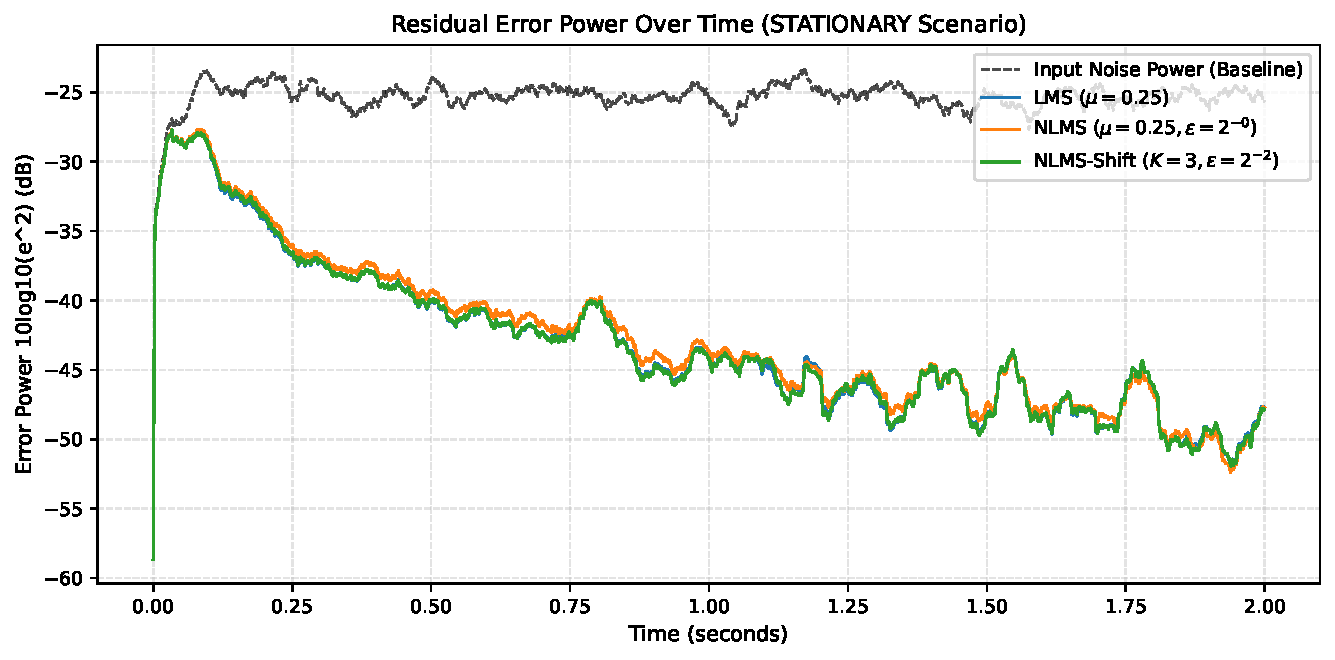
\includegraphics[width=\linewidth]{fig3_residual_error.pdf}
\caption{Residual error power over time compared with the input noise power in the stationary scenario (seed 1).}\label{fig:resid}
\end{figure}
\begin{figure}[!htbp]\centering
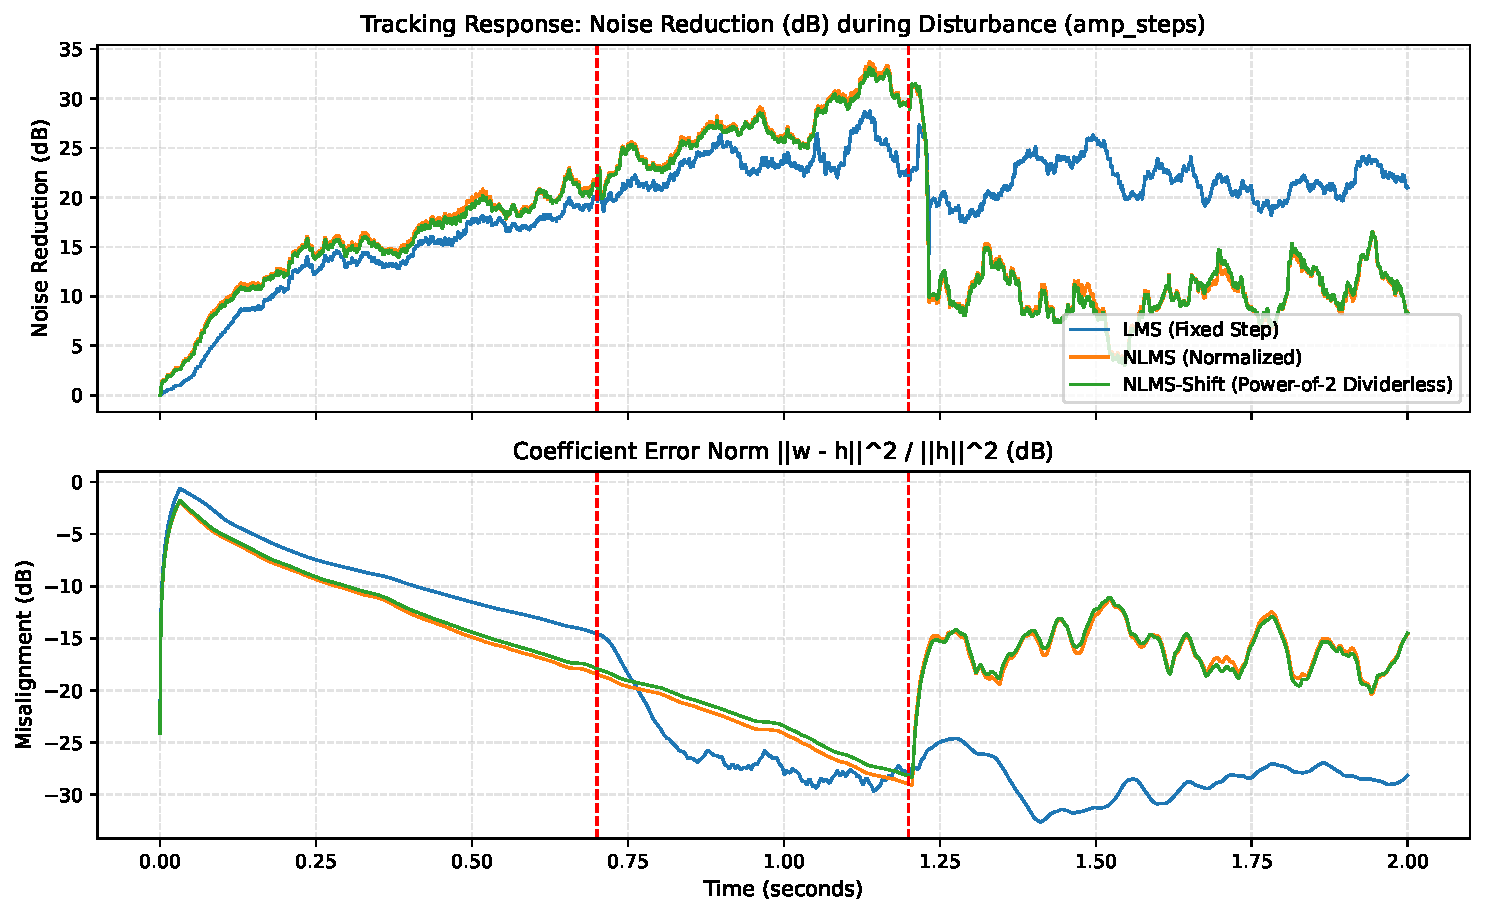
\includegraphics[width=\linewidth]{fig4_tracking_response.pdf}
\caption{Response to the amplitude-step disturbance (seed 1), shown as noise reduction and coefficient misalignment.}\label{fig:track}
\end{figure}

\subsection{Real noise and speech}
\begin{\WT}[!htbp]\centering\small
\caption{Real recorded noise and speech (MS-SNSD), fixed point $W=12$, mean $\pm$ 95\% CI over 20 seeds, no
speech leakage into the reference; STOI and PESQ of $e$ against $s$, with the unprocessed input in brackets
(\texttt{results/metrics/real\_audio\_summary.csv}).}\label{tab:real}
\fitwide{\begin{tabular}{llccc}\toprule
Noise & Metric & LMS & NLMS & NLMS-Shift\\\midrule
\multirow{3}{*}{Air conditioner} & NR (dB) & 11.65 $\pm$ 0.75 & 12.04 $\pm$ 0.82 & 11.89 $\pm$ 0.80\\
 & STOI (input 0.784) & 0.948 & 0.947 & 0.948\\
 & PESQ (input 1.54) & 2.34 & 2.30 & 2.33\\\addlinespace
\multirow{3}{*}{Vacuum cleaner} & NR (dB) & 14.32 $\pm$ 0.32 & 14.90 $\pm$ 0.33 & 14.56 $\pm$ 0.35\\
 & STOI (input 0.730) & 0.982 & 0.983 & 0.982\\
 & PESQ (input 1.39) & 2.81 & 2.81 & 2.81\\\addlinespace
\multirow{3}{*}{Copy machine} & NR (dB) & 14.02 $\pm$ 0.38 & 14.63 $\pm$ 0.34 & 14.39 $\pm$ 0.32\\
 & STOI (input 0.694) & 0.977 & 0.978 & 0.977\\
 & PESQ (input 1.36) & 2.74 & 2.75 & 2.73\\\addlinespace
\multirow{3}{*}{Babble} & NR (dB) & 11.95 $\pm$ 0.42 & 12.43 $\pm$ 0.49 & 12.27 $\pm$ 0.46\\
 & STOI (input 0.719) & 0.956 & 0.955 & 0.955\\
 & PESQ (input 1.48) & 2.48 & 2.47 & 2.47\\
\bottomrule\end{tabular}
}
\end{\WT}
The real recordings (Table~\ref{tab:real}) give a consistent picture across all four noises. Processing
roughly doubles PESQ and brings STOI close to 1, and the order of the algorithms never changes: NLMS leads
LMS by 0.4--0.6~dB, and NLMS-Shift trails NLMS by 0.15--0.35~dB. The noise reduction itself is lower than
in Table~\ref{tab:nr}. It would be easy to blame the real noise for being harder to predict, but that is
not what happens. With the speech removed from the primary input, the same filters on the same noise
segments and paths reached 18.5--19.2~dB on the air conditioner and 22.4--31.9~dB on the other three
noises, which matches or exceeds what they achieve on synthetic stationary noise
(\texttt{py/\allowbreak exp\_real\_audio\_nospeech.py}, \texttt{results/\allowbreak metrics/\allowbreak real\_audio\_nospeech.csv}).
The speech is uncorrelated with the reference, yet it still reaches the error $e[n]$ that drives the
weight update, and that costs 6.4--17.9~dB. LMS suffers most from it. Without speech, LMS is ahead of both
normalized variants on all four noises; with speech, it loses the most (7.6--17.9~dB, against
6.4--14.8~dB for NLMS), so the order flips.

The standard cure is to slow down or halt adaptation during speech. In ULLAP the core's \texttt{freeze}
input (Section~\ref{sec:core}) could be driven by a voice-activity detector for this, but such a detector
has not been tried here. Leakage of speech into the reference is the other practical concern. At
$-20$~dB of leakage the filter starts to cancel part of the speech: noise reduction drops by
2.3--4.6~dB, PESQ by 0.25--0.6, and saturation events show up (18,500 over 19.2 million processed
samples, most of them with the air conditioner). Where the reference microphone is placed therefore
matters more than the choice of algorithm (\texttt{paper/tab\_real\_audio\_xt.tex}).

\subsection{Word length}
Fig.~\ref{fig:wl} shows how much each algorithm loses against its own floating-point version as the word
gets shorter, taking the worst scenario at the tuned settings. The loss is 4.1--5.9~dB at $W=10$,
0.9--1.2~dB at $W=11$ and 0.3--0.4~dB at $W=12$. Eleven bits would already meet the 3~dB criterion; the
design uses 12 to keep some margin. The tonal chord recording is the exception. On it, the fixed-point
filter is up to 3.4~dB better than floating point at $W=11$ and 1.3~dB worse at $W=13$. With so narrow a
band, quantization changes the effective adaptation, so the chord result moves around with the word
length and says little about which word length to choose.

\begin{\WF}[!htbp]\centering
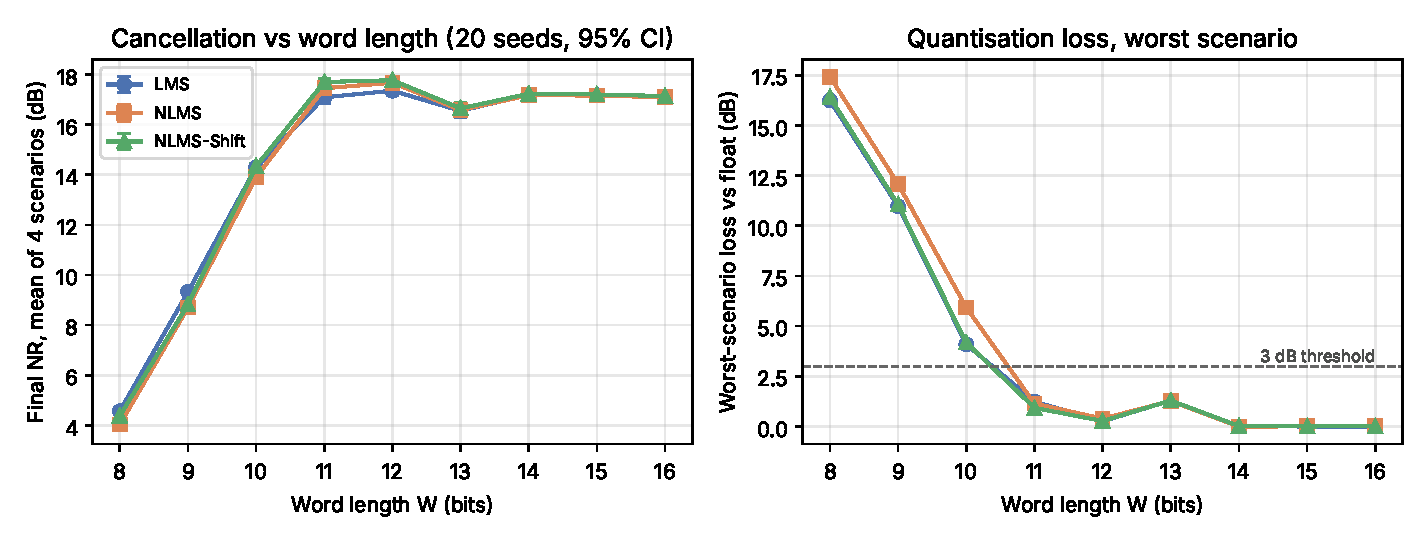
\includegraphics[width=\linewidth]{fig13_wordlength_fair.pdf}
\caption{Noise reduction and worst-scenario quantization loss versus word length (20 seeds).}\label{fig:wl}
\end{\WF}

\subsection{Equivalent step size of NLMS-Shift}\label{sec:equiv}
Equation~\eqref{eq:ratio} says that NLMS-Shift is NLMS with an extra factor $r[n]$ in the step. If input
levels are spread evenly on a logarithmic scale, this factor averages to
$E[r]=\int_0^1 2^{u-1}\,du=1/(2\ln 2)\approx0.72$. At any particular level, however, $r$ depends on where
$P+\epsilon$ sits inside its octave. It grows with the level and drops by half each time $P+\epsilon$
crosses a power of two. For $L=32$ and $\epsilon=2^{-2}$, the crossing at $P+\epsilon=1/2$ corresponds to
a reference RMS of $-21.1$~dBFS, only 3~dB above the level used in the simulations. The integer model was
used to see what this does in practice (\texttt{py/exp\_equiv\_step.py}): the input level was swept over
12~dB in steps of 0.75~dB, once on the stationary scenario (seeds 1--5) and once with a two-tone reference
(Fig.~\ref{fig:equiv}).

Broadband noise makes the window power fluctuate enough to smear out the sawtooth, and the mean ratio
$\bar r$ drifts smoothly between 0.56 and 0.78. The two-tone reference behaves differently. Its power $P$
is almost constant, and $\bar r$ falls from 0.87 to 0.62 within a single 0.75~dB step of level. In both
cases, plain NLMS run with the constant step $\bar r\,2^{-K}$ behaves like NLMS-Shift. Their final noise
reduction agrees within 0.27~dB at all 17 broadband levels; for the tones it agrees within 0.55~dB at
every level except the one that straddles the crossing (1.7~dB). Convergence times agree within 8\%. NLMS
with the nominal step $2^{-K}$, by comparison, is off by as much as 3.5~dB and 48\%.

The shift, in short, touches only the step size. Instead of a fixed NLMS step, the filter gets a step
between $0.5$ and $1$ times the nominal one, and the input level decides where in that range it falls.
With broadband input the result is a gentle change of gain, which is absorbed by choosing $K$ (and
$\epsilon$) for the level the system expects. Tonal input is less forgiving: whenever its level crosses a
power-of-two boundary of $P+\epsilon$, the step changes by up to a factor of about 0.7. A fixed-step NLMS
never does this.
\begin{figure}[!htbp]\centering
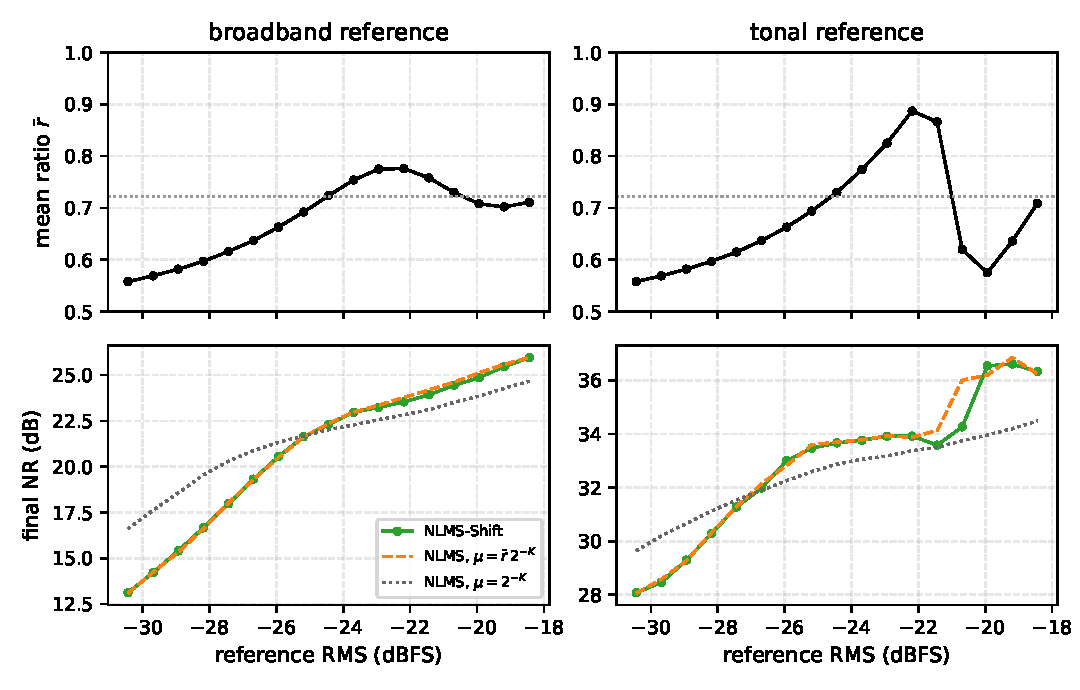
\includegraphics[width=\linewidth]{fig16_equiv_step.pdf}
\caption{Equivalent step of NLMS-Shift versus reference level (integer model, $W=12$, $L=32$, $K=3$,
$\epsilon=2^{-2}$). Top: mean ratio $\bar r$ of \eqref{eq:ratio}; dotted: $1/(2\ln2)$. Bottom: final noise
reduction of NLMS-Shift, of NLMS with step $\bar r\,2^{-K}$ and of NLMS with step $2^{-K}$. Left:
stationary scenario, seeds 1--5; right: two-tone reference (\texttt{results/metrics/equiv\_step.csv}).}\label{fig:equiv}
\end{figure}

\subsection{Hardware cost}
\begin{table}[!htbp]\centering\small
\caption{Complete board design (core, codec interface, synchronizers, status logic) on Cyclone IV E
EP4CE115F29C7, $W=12$, $L=32$, Quartus Prime Lite 25.1, commit da0b6f4
(\texttt{results/quartus\_reports/board\_da0b6f4/}, \texttt{results/metrics/power\_activity.csv}).}\label{tab:hw}
\fitcol{\begin{tabular}{lccc}\toprule
 & LMS & NLMS & NLMS-Shift\\\midrule
Logic elements & 1,792 & 2,626 & 2,610\\
Registers & 1,123 & 1,404 & 1,186\\
9-bit multipliers & 4 & 4 & 4\\
$F_{\max}$, slow 85\,$^\circ$C (MHz) & 70.08 & 59.75 & 58.66\\
Setup slack at 50~MHz, slow 85\,$^\circ$C (ns) & 5.731 & 3.263 & 2.953\\
Latency (cycles) & 35 & 37 & 37\\
Busy cycles per sample (measured on the board) & 73 & 130 & 72\\
RTL bit toggles per sample & 5,668 & 7,146 & 6,012\\
Core dynamic power, vectorless (mW) & 20.79 & 24.36 & 23.77\\\bottomrule
\end{tabular}}
\end{table}
Table~\ref{tab:hw} gives the cost of the complete board design. LMS needs about 31\% less logic than
either normalized variant. Between NLMS-Shift and NLMS there is almost nothing to choose in logic elements
(2,610 against 2,626): what the shift saves by dropping the divider, it spends again on the leading-one
detector, the shifter and a wider update path. NLMS-Shift gains in other respects. It has 15\% fewer
registers, needs 45\% fewer busy cycles per sample and toggles 16\% fewer bits per sample. Timing is not
an issue for any of the three. Each meets the 50~MHz constraint with at least +2.953~ns of setup slack and
+0.401~ns of hold slack, and Quartus reports no critical warnings. At 8.138~kHz even the busiest variant
is active for only 2\% of the 6,144-cycle sample period, so one core could handle many channels or much
longer filters.

The power numbers in Table~\ref{tab:hw} need some care. They are vectorless Quartus estimates at the
default toggle rate of 12.5\%, and Quartus itself grades them as low confidence. Most of the 169 to
173~mW total is core static power (about 98.7~mW). The dynamic part ranks the designs LMS $<$ NLMS-Shift
$<$ NLMS, which is also the order of the toggle counts. A fixed toggle rate, though, mainly reflects area.
It has no way of knowing that the datapath sits idle for 98\% of each sample period, so the figures are
upper bounds and not energy per sample. A gate-level estimate with real switching activity is left for
future work; it needs a separate netlist-only testbench, because the post-fit netlist flattens the
hierarchy that the top-level testbench looks into. The same missing number stands in the way of a fair
comparison with Huang and Yao~\cite{huang2026}, who worked on the same board. Such a comparison would use
energy per sample, i.e.\ the dynamic power from an activity-annotated Power Analyzer run divided by the
sample rate. Until that figure exists, no energy comparison with their design is claimed. Even then, area
and energy would have to be compared per tap and per sample rather than as raw totals, since their design
is fully parallel and runs at megasamples per second, while ULLAP shares a single multiplier and runs at
8.138~kHz.



\subsection{On-board results}\label{sec:board}
All board measurements were taken with Signal Tap, the logic analyzer embedded in the FPGA tool flow, so
no external recorder or oscilloscope was involved. One analyzer instance stores three values once per
sample: the two codec samples entering the core ($x$ and $d$, from the registers \texttt{x\_reg} and
\texttt{d\_reg}) and the core output $e$. A transitional storage qualifier on \texttt{out\_valid} picks out
one entry per sample; the trigger is the release of the reset button, and the buffer holds 32,768 samples
(4.0~s). A second instance watches the four GPIO test points at 50~MHz. For the stimuli, the noise-only
versions of the four scenarios were played from a laptop into LINE IN, each preceded by a 1~kHz
calibration tone. Reset was pressed while the tone was playing. Every capture therefore starts with zero
weights on real codec data at about $-25$~dBFS, and no captured sample reaches full scale. The analysis
script and the raw exports are kept in the repository (\texttt{py/analyze\_board\_capture.py},
\texttt{board\_evidence/}).

\emph{Bit-exactness.} The check itself is simple. For each of the 12 captures (three algorithms times four
scenarios), the integer model of Section~\ref{sec:model} was started from zero state at the first sample
after reset, given the captured $x$ and $d$, and left to compute $e[n]$. Its output matched the captured
$e[n]$ sample for sample, with no mismatch anywhere in 351,723 samples (28,672 to 32,768 per capture, or
3.5 to 4.0~s). The chip, in other words, computes exactly the fixed-point arithmetic that was evaluated in
simulation, and it does so on analog input carrying the codec's noise and offsets.

\emph{Timing.} The GPIO capture gives an \texttt{in\_valid} period of 6,144 clock cycles, i.e.\
8,138.02~Hz. From \texttt{in\_valid} to \texttt{out\_valid} it measures 38, 36 and 38 cycles for
NLMS-Shift, LMS and NLMS (0.76, 0.72 and 0.76~$\mu$s); this is the core latency plus one cycle to accept
the sample. The busy times are 72, 73 and 130 cycles. Every one of these values is the same as in RTL
simulation with identical parameters. Adding Signal Tap does not break timing either: those builds still
meet 50~MHz, with setup slack of $+2.65$, $+5.68$ and $+3.78$~ns. (Table~\ref{tab:hw} refers to the builds
without the logic analyzer.)

Fig.~\ref{fig:board} puts the three algorithms side by side on the same amplitude-step stimulus, aligned
to the start of the scenario. Because KEY0 was pressed by hand during the calibration tone, the reset
falls at a slightly different point of the stimulus in each capture. All three reach about 15~dB within
the first 1.5~s. At 2.1~s the level of $d$ jumps by 7.4~dB, and the filters follow with only a short burst
in $e$. After the step, the residual power ($-47$ to $-52$~dBFS) is actually lower than before it
($-44$~dBFS), and the noise reduction rises to 25 to 30~dB. Over the last quarter of the window, about
40~dB is removed below 1.5~kHz and 11 to 15~dB near the band edge (3.5 to 3.9~kHz).

\emph{Noise reduction on the simulation signal.} In a second session the board was fed exactly the
signals used in the simulations, so that its noise reduction could be compared with the model directly.
For each scenario, the 2~s, seed-1 noise-only signal (the same 16,000 samples as in the simulations) was
played once after the calibration tone, which lets the whole scenario fit in one capture. Correlating the
captured $x$ with the stimulus located its start (correlation 0.95 to 0.99), and
$\mathrm{NR}_\mathrm{final}$ was taken over the same last 25~\% as in simulation. All 12 captures, 28,672
samples after reset each, are bit-exact once again.

Table~\ref{tab:board} sets board and integer model against each other on the same signal. The board ends
up 2.9 to 10.6~dB below the simulation, by about the same amount for all three algorithms. The hardware is
not the cause; the input level is. The codec delivered $x$ and $d$ at about $-27$~dBFS, 3~dB lower than in
simulation, and with the tuned step sizes a quieter input adapts more slowly within the 2~s. When the
model is fed the level the board actually received, it agrees with the board to within 0.2~dB on
stationary and path-switch noise (Fig.~\ref{fig:boardlevel}). The amplitude-step and recorded-noise
scenarios are harder to match because their final quarter is quiet ($d$ near $-41$ and $-57$~dBFS), and
there the board stays 1.7 to 8.1~dB below the level-matched model. At such low levels two analog effects
start to matter next to $d$: the noise of the playback and codec chain ($-70$~dBFS, measured in the
silence after the stimulus) and an ADC offset that dies away during the first second after reset. A
simple check on the amplitude-step window shows how much this limits the result. Even the best 32-tap
least-squares filter fitted to the board samples of that window reaches only 24~dB, against 28~dB on the
ideal signal. Across all scenarios on the board, the three algorithms stay within 0.7~dB of one another.

\begin{table}[!htbp]\centering\small
\caption{On-board $\mathrm{NR}_\mathrm{final}$ (dB) on the 2~s seed-1 stimulus against the integer model on
the same signal, at the simulation level and scaled to the level the board received
(\texttt{results/board/session2/}). Every board capture is bit-exact.}\label{tab:board}
\fitcol{\begin{tabular}{llrrr}\toprule
Algorithm & Scenario & Board & Model, sim.\ level & Model, board level\\\midrule
LMS & stationary & 15.88 & 22.77 & 15.76\\
 & amplitude steps & 17.13 & 27.71 & 25.23\\
 & path switch & 14.67 & 19.84 & 14.47\\
 & recorded noise & 5.99 & 9.11 & 7.78\\\midrule
NLMS & stationary & 15.65 & 21.60 & 15.53\\
 & amplitude steps & 16.76 & 27.19 & 23.64\\
 & path switch & 14.03 & 19.06 & 14.04\\
 & recorded noise & 5.80 & 8.72 & 7.45\\\midrule
NLMS-Shift & stationary & 15.80 & 22.68 & 15.78\\
 & amplitude steps & 16.57 & 25.79 & 22.10\\
 & path switch & 14.40 & 19.86 & 14.44\\
 & recorded noise & 5.46 & 8.63 & 7.32\\\bottomrule
\end{tabular}}
\end{table}

\begin{\WF}[!htbp]\centering
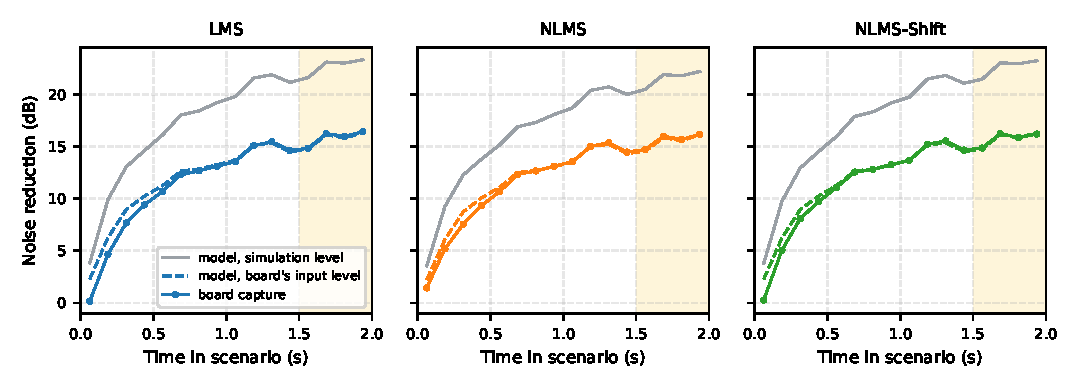
\includegraphics[width=\linewidth]{fig15_board_vs_model_stationary.pdf}
\caption{Running noise reduction (0.125~s windows) on the 2~s stationary stimulus: board capture, integer
model at the simulation level, and integer model with the stimulus scaled to the level the board
received. Shaded: the $\mathrm{NR}_\mathrm{final}$ window.}\label{fig:boardlevel}
\end{\WF}

\emph{Freeze, DAC word and endurance.} To test the freeze path, SW[1] was flipped by hand 1.44~s into a
stationary-noise run with NLMS-Shift. The captured output equals the model with adaptation stopped from
that sample onwards (28,672 samples, no mismatch). From the switch to the end of the run, the noise
reduction holds at 15.2~dB; just before the switch it was 15.4~dB, and with adaptation left running it
would have been 15.9~dB. A third Signal Tap instance looked at the word sent to the DAC. In ANC mode this
word is $\{e, 0000\}$, and in bypass ($\mathrm{SW}[0]=1$) its upper 12 bits are $d$, in all 1,792 samples
of each capture. The analog LINE OUT signal could not be recorded with the equipment available, so the
check ends at the DAC interface. Finally, the board was left running for 10~minutes on looped noise.
Afterwards the GPIO timing was unchanged (6,144 cycles per sample, 38 cycles from \texttt{in\_valid} to
\texttt{out\_valid}, 72 busy cycles), and none of the saturation, NACK or overrun flags had been set. With
all three analyzer instances included, the build still met timing (slack $+2.93$~ns).

\begin{\WF}[!htbp]\centering
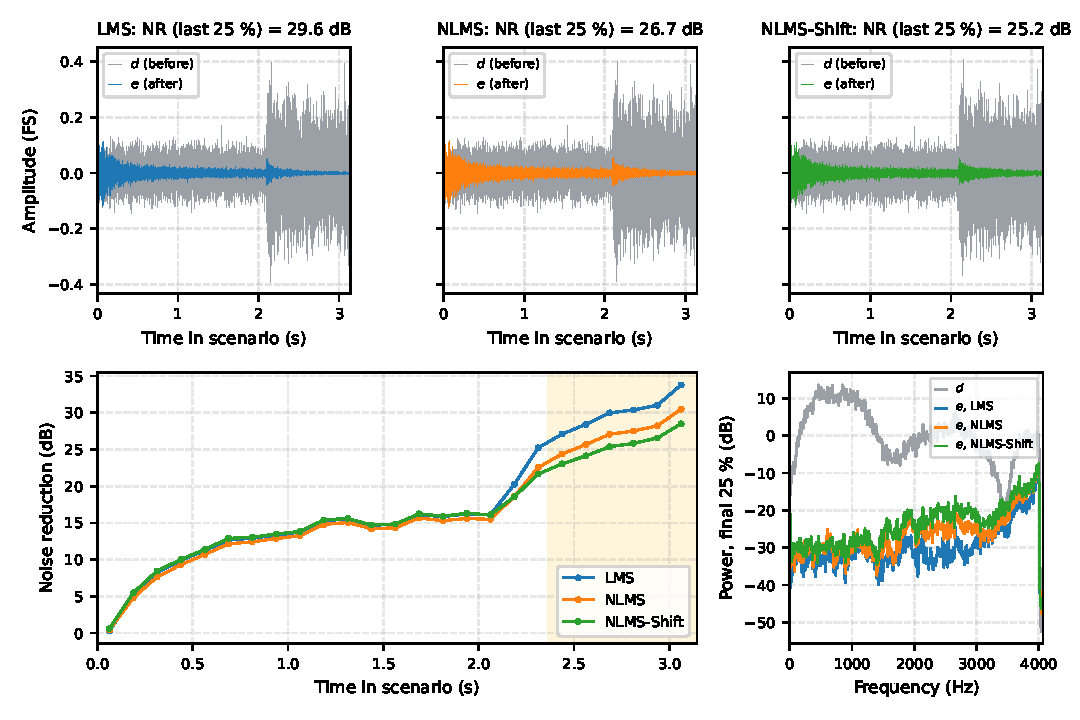
\includegraphics[width=\linewidth]{fig14_board_capture_amp_steps.pdf}
\caption{On-board Signal Tap captures of LMS, NLMS and NLMS-Shift on the same amplitude-step noise, from
the start of the scenario: primary input $d$ and output $e$ (top), running noise reduction in 0.125~s
windows (bottom left; shaded: last 25~\% of the common window) and power spectra over that window
(bottom right). Every output sample of all three captures equals the integer model's.}\label{fig:board}
\end{\WF}

%--------------------------------------------------------------------------------------------
\FloatBarrier % every figure and table is placed before the discussion
\section{Discussion and limitations}\label{sec:disc}
We would state the main finding modestly. Replacing the divider with a shift keeps most of what makes NLMS
useful, its insensitivity to the input level, and brings the cycle count down to about that of LMS (72
against 73 busy cycles per sample). If the noise level moves around and throughput or energy per sample
is the scarce resource, NLMS-Shift is the sensible pick; with a steady level, plain LMS is still the
smallest circuit. What the data do not show is NLMS-Shift cancelling better than NLMS, and
Section~\ref{sec:equiv} explains why not: the shift only rescales the step, by a factor somewhere between
0.5 and 1 that depends on the input level. Getting $K$ and $\epsilon$ right for the level the system will
actually see is worth more than the shift itself. The one quirk is tonal noise sitting near a power-of-two
boundary of $P+\epsilon$, where the step can jump in a way NLMS never would. On real recordings the bigger
story is the speech. It costs all three algorithms 6.4--17.9~dB, while the algorithms differ from one
another by 0.6~dB at most.

Some caveats. Every acoustic path in this study is simulated, even where the noise and speech are real
recordings. Howling from closed-loop acoustic feedback is not addressed at all; a reference-based canceller
is the wrong tool for that problem anyway. Our power numbers are a switching-activity proxy and will stay
that way until a gate-level analysis is run. On the board we followed the samples as far as the DAC word
but never recorded the analog LINE OUT signal. And the absolute noise reduction is sensitive to input
level. With the stimulus 3~dB quieter than in simulation, the board managed 14 to 17~dB on the synthetic
scenarios rather than 19 to 28~dB, a drop the model reproduces at that level for stationary and
path-switch noise. Anyone building on this design should set the codec input gain so the reference uses
most of the 12-bit range, or else retune the step size for the level they expect.

\section{Conclusion}\label{sec:concl}
The question behind ULLAP was a practical one: on a cheap FPGA with one shared multiplier and 12-bit
words, what does a fair comparison of LMS, NLMS and NLMS-Shift look like, and does the chip really compute
what the model predicts? Running all three on the same serial 32-tap core, tuned with equal effort, gives
a fairly clear answer. NLMS-Shift stays within the 95\% confidence interval of NLMS on stationary and
amplitude-step noise, and gets there in 72 busy cycles per sample where NLMS needs 130. Analytically it is
NLMS with a step that wanders between 0.5 and 1 times the nominal value as the level changes, nothing
more. Real recordings tell a second story. All three filters remove 11.7 to 14.9~dB of real noise when
speech is present and 18.5 to 31.9~dB when it is not, so the speech, not the noise, is what holds them
back. Finally, the hardware does what the model says. Twenty-five Signal Tap captures of real codec data,
724,459 samples in all, match the integer model bit for bit, and so do the freeze behavior and the DAC
word; on stationary and path-switch noise the measured noise reduction agrees with the model, at the level
the board actually received, within 0.2~dB.

\section*{Declarations}
\decl{Funding} \TBD{Authors: funding sources, or ``No funding was received for this work.''}

\decl{Competing interests} \TBD{Authors: competing interests, or ``The authors declare no
competing interests.''}

\decl{Author contributions} \TBD{Authors: who did what (free text or CRediT).}

\decl{Data and code availability}
All RTL, testbenches, scripts and result files are available in the project repository
\TBD{public URL and Zenodo DOI of the tagged release}. The real-audio study downloads its MS-SNSD files
from a pinned commit and verifies them by SHA-256.

\decl{Use of generative AI} Described in the experimental set-up (Section~\ref{sec:setup}).


\bibliographystyle{IEEEtran}
\bibliography{refs}
\end{document}
